\mode*

% Since this a solution template for a generic talk, very little can
% be said about how it should be structured. However, the talk length
% of between 15min and 45min and the theme suggest that you stick to
% the following rules:  

% - Exactly two or three sections (other than the summary).
% - At *most* three subsections per section.
% - Talk about 30s to 2min per frame. So there should be between about
%   15 and 30 frames, all told.


\section{The Big Picture}

\begin{frame}
  \begin{center}
    Detection
    \qquad
    \textbf{Prevention}
    \qquad
    Recovery
  \end{center}
\end{frame}


\section{Firewalls}

\begin{frame}
  \begin{figure}
    \includegraphics[height=0.70\textheight]{figs/network-rotated.pdf}
    \caption{Example network topology.
      Two remote workers, one hacker and two servers connected over the 
      Internet.
      Three servers, four offices on the internal network.
    }
  \end{figure}
\end{frame}

\begin{frame}
  \centering
  \includegraphics[height=0.60\textheight]{figs/network-rotated.pdf}

  \only<1>{
    \begin{definition}[Firewall]
      \begin{itemize}
        \item A firewall enforces certain traffic flows.
      \end{itemize}
    \end{definition}
  }
  \only<2>{
    \begin{example}[Firewall]
      \begin{itemize}
        \item Prevent outsiders from establishing connections to insiders.
        \item Insiders may establish connections to outsiders though.
      \end{itemize}
    \end{example}
  }
\end{frame}

\begin{frame}
  \centering
  \includegraphics[height=0.60\textheight]{figs/network-rotated.pdf}

  \only<1>{
    \begin{definition}[Network-based intrusion detection]
      \begin{itemize}
        \item Analyses events generated by network communication patterns.
        \item Internal and going outside.
      \end{itemize}
    \end{definition}
  }
  \only<2>{
    \begin{example}[Network-based intrusion detection]
      \begin{itemize}
        \item Connection from laptop to server.
        \item Immediately followed by connection to outside.
      \end{itemize}
    \end{example}
  }
\end{frame}


\section{Packet filters}

\begin{frame}
  \begin{figure}
    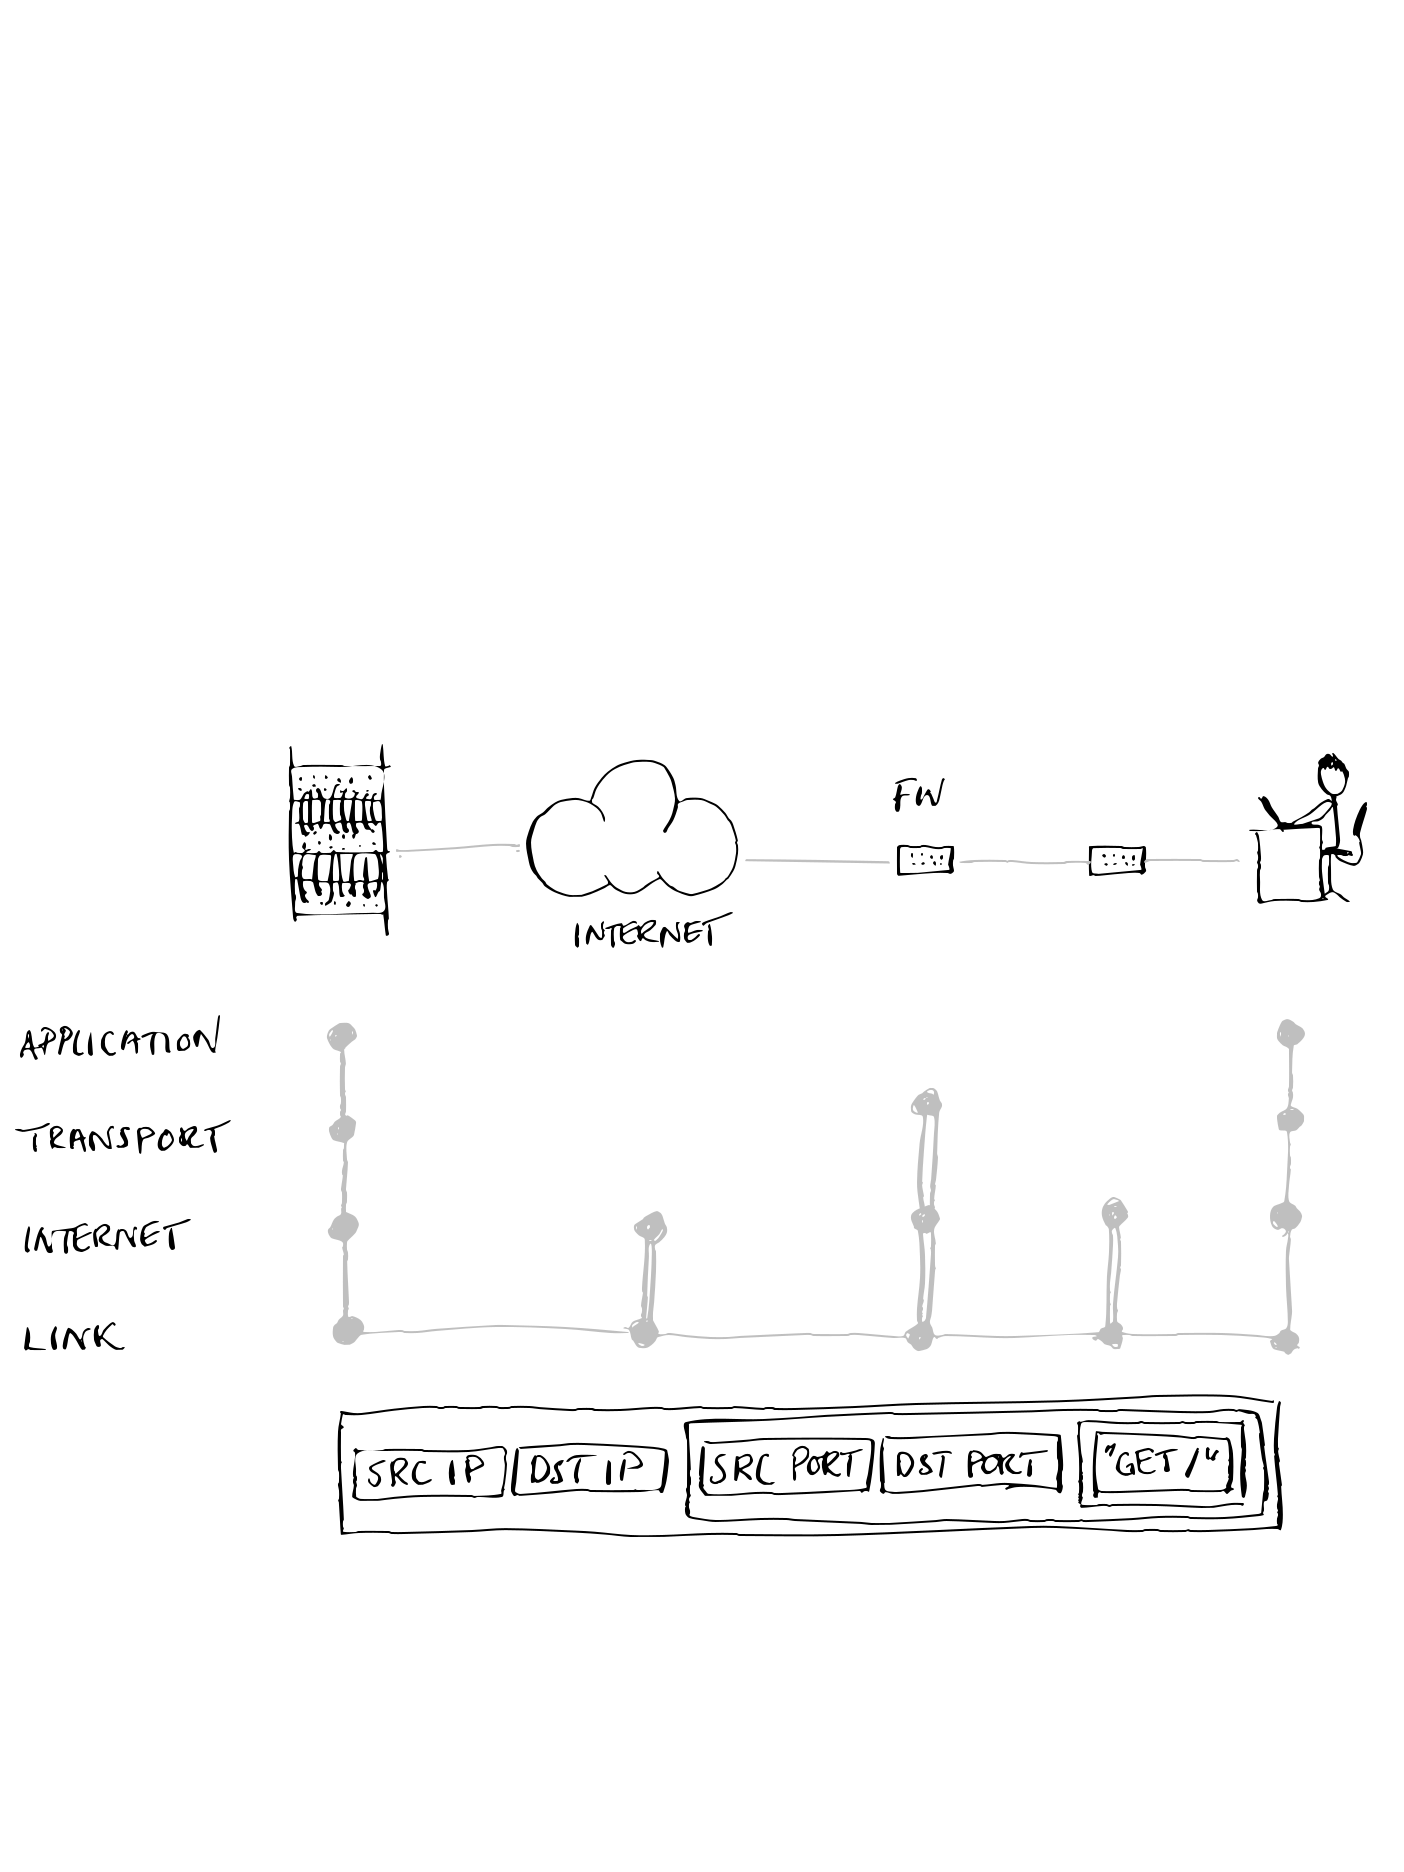
\includegraphics[width=\columnwidth]{figs/network-layers-fw.pdf}
    \caption{Communication between Bob and a server.}
  \end{figure}
\end{frame}

\begin{frame}[fragile]
  \begin{definition}[Packet filter]
    \begin{itemize}
      \item \emph{Stateless} filtering based on transport layer data.
    \end{itemize}
  \end{definition}

  \begin{minted}{json}
    {
      "src addr": "Bob",
      "dst addr": "server",
      "payload": {
        "src port": "random",
        "dst port": "https",
        "payload": "unintelligible blob"
      }
    }
  \end{minted}
\end{frame}

\begin{frame}
  \begin{definition}[Ingress, egress filtering]
    \begin{description}
      \item[Ingress] inbound traffic.
      \item[Egress] outbound traffic.
    \end{description}
  \end{definition}
\end{frame}

\begin{frame}[fragile]
  \begin{example}[Ingress filtering]
  \begin{minted}{json}
    {
      "src addr": "not internal",
      "dst addr": "Bob",
      "payload": {
        "src port": "random",
        "dst port": "https",
        "payload": "unintelligible blob"
      }
    }
  \end{minted}
  \end{example}
\end{frame}

\begin{frame}[fragile]
  \begin{example}[Egress filtering]
  \begin{minted}{json}
    {
      "src addr": "Bob",
      "dst addr": "server",
      "payload": {
        "src port": "random",
        "dst port": "http",
        "payload": "unintelligible blob"
      }
    }
  \end{minted}
  \end{example}
\end{frame}

\begin{frame}
  \begin{remark}
    \begin{itemize}
      \item A blunt tool.
      \item Discard or forward a packet.
      \item Vulnerable to TCP/IP bugs.
    \end{itemize}
  \end{remark}
\end{frame}


\section[SPI]{Circuit-level gateways}

\begin{frame}[fragile]
  \begin{definition}[Stateful firewall/circuit-level gateway]
    \begin{itemize}
      \item Stateful filtering based on transport layer data.
    \end{itemize}
  \end{definition}

  \begin{columns}[T]
    \begin{column}{0.35\columnwidth}
      \begin{minted}{json}
    {
      "src addr": "Bob",
      "dst addr": "server",
      "payload": {
        "flag": "SYN",
        "seq num": 0,
        "src port": "random",
        "dst port": "https",
        "payload": "blob"
      }
    }
      \end{minted}
    \end{column}
    \begin{column}{0.55\columnwidth}
      \begin{tabular}{llll}
        \textbf{src} & \textbf{dst} & \textbf{state} & \textbf{sn} \\
        \midrule
        Bob:random & server:https & SYN & 0
      \end{tabular}
    \end{column}
  \end{columns}
\end{frame}

\begin{frame}[fragile]
  \begin{columns}[T]
    \begin{column}{0.35\columnwidth}
      \begin{minted}{json}
    {
      "src addr": "server",
      "dst addr": "Bob",
      "payload": {
        "flag": "ACK",
        "seq num": 1,
        "src port": "https",
        "dst port": "random",
        "payload": "blob"
      }
    }
      \end{minted}
    \end{column}
    \begin{column}{0.55\columnwidth}
      \begin{tabular}{llll}
        \textbf{src} & \textbf{dst} & \textbf{state} & \textbf{sn} \\
        \midrule
        Bob:random & server:https
                   & \only<1>{SYN}\only<2>{\color{blue}ACK}
                   & \only<1>{0}\only<2>{\color{blue}1}
      \end{tabular}
    \end{column}
  \end{columns}
\end{frame}

\begin{frame}
  \begin{remark}
    \begin{itemize}
      \item Keeps track of TCP connections.
      \item Avoids TCP/IP bugs.
    \end{itemize}
  \end{remark}
\end{frame}


\section[DPI]{Application firewalls}

\begin{frame}
  \begin{figure}
    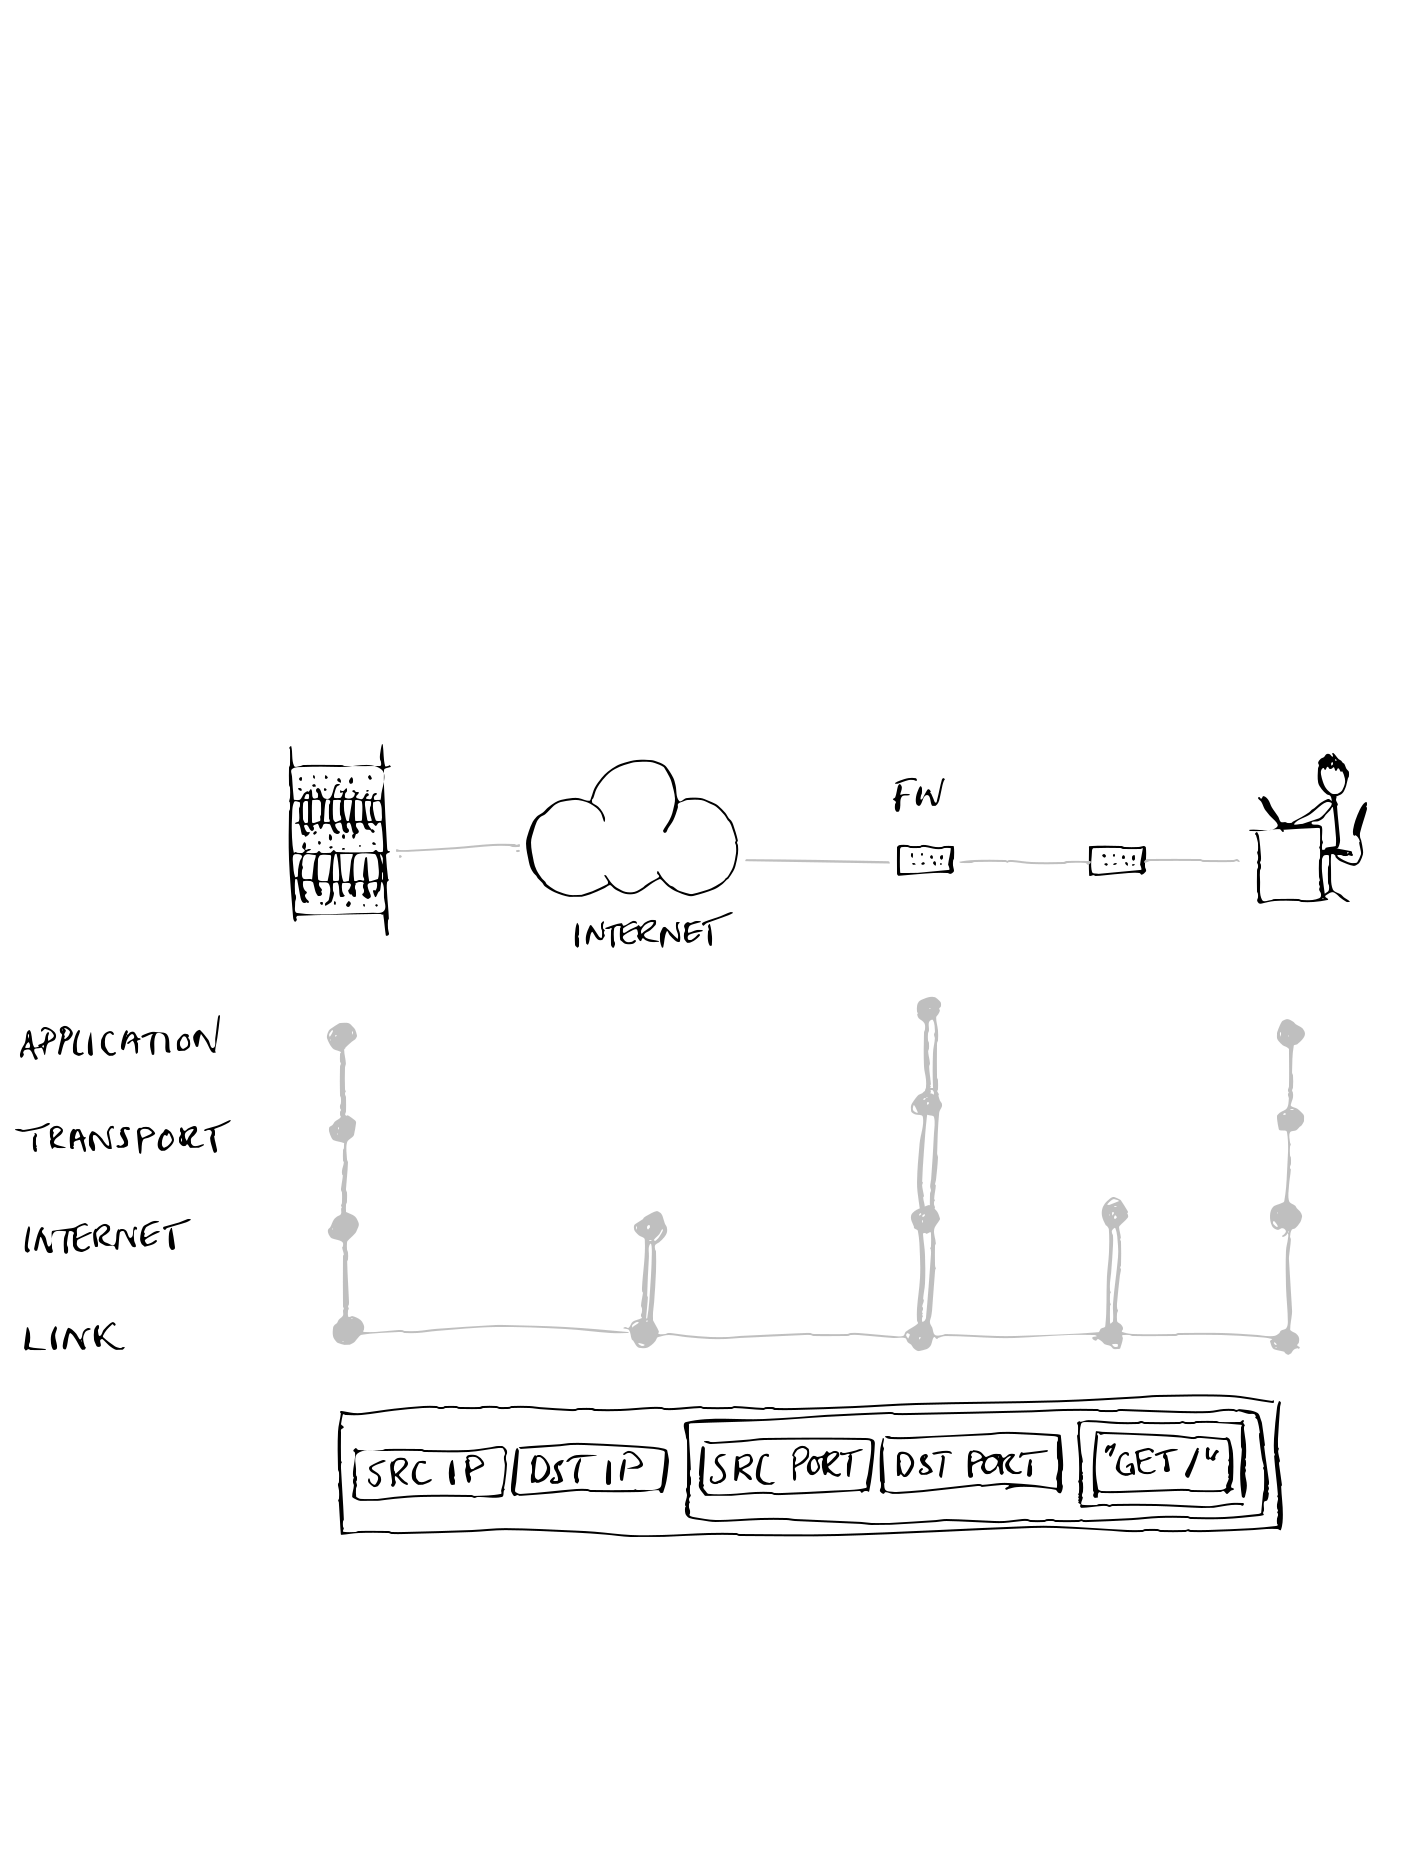
\includegraphics[width=\columnwidth]{figs/network-layers-dpi.pdf}
    \caption{Communication between Bob and a server.}
  \end{figure}
\end{frame}

\begin{frame}[fragile]
  \begin{definition}[Application firewalls/Deep packet inspection]
    \begin{itemize}
      \item Stateful filtering based on data from \emph{all layers}.
    \end{itemize}
  \end{definition}
  \begin{minted}{json}
    {
      "src addr": "server",
      "dst addr": "Bob",
      "payload": {
        "flag": "ACK",
        "seq num": 4,
        "src port": "http",
        "dst port": "random",
        "payload": {
          "data": "...<h1>Down with government!</h1>..."
        }
      }
    }
  \end{minted}
\end{frame}

\begin{frame}
  \begin{remark}
    \begin{itemize}
      \item Can detect banned content.
      \item Can detect forbidden protocols on non-standard ports.
      \item Can even detect certain buffer-overflow attacks.
      \item Essentially a combination of stateful firewall and network-based 
        intrusion detection system.
    \end{itemize}
  \end{remark}
\end{frame}

\begin{frame}
  \begin{example}[The Great Firewall of China]
    \begin{itemize}
      \item Many countries engaging in censorship use DPI.
      \item See 
        \citetitle{MeasuringCircumventingInternetCensorship}\footfullcite{MeasuringCircumventingInternetCensorship} 
        for an adversarial treatment of DPI.
    \end{itemize}
  \end{example}
\end{frame}


\section{Placement}

\begin{frame}
  \centering
  \only<1>{
    \includegraphics[height=0.70\textheight]{figs/network-rotated.pdf}
  }
  \only<2>{
    \includegraphics[height=0.70\textheight]{figs/network-dmz-rotated.pdf}
  }

  \begin{question}
    \begin{itemize}
      \item Where to place the firewall?
    \end{itemize}
  \end{question}
\end{frame}

\begin{frame}
  \begin{block}{Types}
    \begin{description}
      \item[Bastion host] Stronghold in network.
        \begin{itemize}
          \item Minimize attack surface.
        \end{itemize}

      \item[Host based] Firewalls on servers, secure individual host.
        \begin{itemize}
          \item Tailored filter to host needs.
          \item Protects from internal attacks.
        \end{itemize}

      \item[Personal] Firewall on workstations, much less complex.
    \end{description}
  \end{block}
\end{frame}

